\item \textbf{For each dataset, examine the stationarity of the residuals using the ACF and PACF functions, Lag Plots, and/or other approaches. Show your results and provide commentary about your observations.}

\textit{\gls{ADF} shows that the time series is non-stationary or stationary. If the p-value is less than the significance level of 0.05 and the \gls{ADF} statistic is lower than one of the critical values, then the time series is stationary. For example, tables \ref{tab:Ass1_D1_ADF} and \ref{tab:Ass1_D2_ADF} shows the result of \gls{ADF} on a residual component of STL method in the two datasets.}

\begin{table}[H]
\centering
\caption{The result of the \gls{ADF} on the first dataset.}
\label{tab:Ass1_D1_ADF}
\begin{tabular}{lr}
\toprule
{} &            0 \\
\midrule
ADF Statistic               &   -24.697687 \\
p-value                     &     0.000000 \\
\#Lags Used                  &     3.000000 \\
Number of Observations Used &  3646.000000 \\
Critical Value (1\%)         &    -3.432145 \\
Critical Value (5\%)         &    -2.862333 \\
Critical Value (10\%)        &    -2.567192 \\
\bottomrule
\end{tabular}

\end{table}

\begin{table}[H]
\centering
\caption{The result of the \gls{ADF} on the second dataset.}
\label{tab:Ass1_D2_ADF}
\begin{tabular}{lr}
\toprule
{} &             0 \\
\midrule
ADF Statistic               & -1.128610e+01 \\
p-value                     &  1.416821e-20 \\
\#Lags Used                  &  2.700000e+01 \\
Number of Observations Used &  2.792000e+03 \\
Critical Value (1\%)         & -3.432694e+00 \\
Critical Value (5\%)         & -2.862576e+00 \\
Critical Value (10\%)        & -2.567321e+00 \\
\bottomrule
\end{tabular}

\end{table}



\textit{\gls{KPSS} is another test for checking the stationarity of a time series. If the p-value is less than the significance level of 0.05, then the time series is not stationary. Table \ref{tab:Ass1_D1_KPSS} and \ref{tab:Ass1_D2_KPSS} show the result of this test on STL residual.}

\begin{table}[H]
\centering
\caption{The result of the \gls{KPSS} on the first dataset.}
\label{tab:Ass1_D1_KPSS}
\begin{tabular}{lr}
\toprule
{} &          0 \\
\midrule
KPSS Statistic        &   0.318117 \\
p-value               &   0.100000 \\
Lags Used             &  22.000000 \\
Critical Value (10\%)  &   0.347000 \\
Critical Value (5\%)   &   0.463000 \\
Critical Value (2.5\%) &   0.574000 \\
Critical Value (1\%)   &   0.739000 \\
\bottomrule
\end{tabular}

\end{table}

\begin{table}[H]
\centering
\caption{The result of the \gls{KPSS} on the second dataset.}
\label{tab:Ass1_D2_KPSS}
\begin{tabular}{lr}
\toprule
{} &          0 \\
\midrule
KPSS Statistic        &   0.017052 \\
p-value               &   0.100000 \\
Lags Used             &  68.000000 \\
Critical Value (10\%)  &   0.347000 \\
Critical Value (5\%)   &   0.463000 \\
Critical Value (2.5\%) &   0.574000 \\
Critical Value (1\%)   &   0.739000 \\
\bottomrule
\end{tabular}

\end{table}

\textit{We can conclude that the series is stationary or not based on both \gls{KPSS} and \gls{ADF} \cite{StationarityStatsmodels}. Table \ref{tab:1} shows the possible outcomes of applying these two tests.}

\begin{table}[H]
\centering
\caption{The combination of the result of the \gls{KPSS} and \gls{ADF}.}
\label{tab:1}
% Please add the following required packages to your document preamble:
% \usepackage[table,xcdraw]{xcolor}
% If you use beamer only pass "xcolor=table" option, i.e. \documentclass[xcolor=table]{beamer}
\centering
\begin{tabular}{|l|l|l|}
\hline
KPSS test      & KDF test       & The combination result                      \\ \hline
non-stationary & non-stationary & The series is non-stationary.               \\ \hline
stationary     & non-stationary & Use detrending to make series stationary.   \\ \hline
non-stationary & stationary     & Use differencing to make series stationary. \\ \hline
stationary     & stationary     & The series is stationary.                   \\ \hline
\end{tabular}

\end{table}



\textit{\gls{ACF} and \gls{PACF} plots allow us to determine how correlated points are with each other. Figures \ref{fig:Ass1_D1_PACF_ACF} and \ref{fig:Ass1_D2_PACF_ACF} indicate these two plots for our datasets. }



\begin{figure}[H]
    \centering
    \begin{minipage}[b]{1\textwidth}
        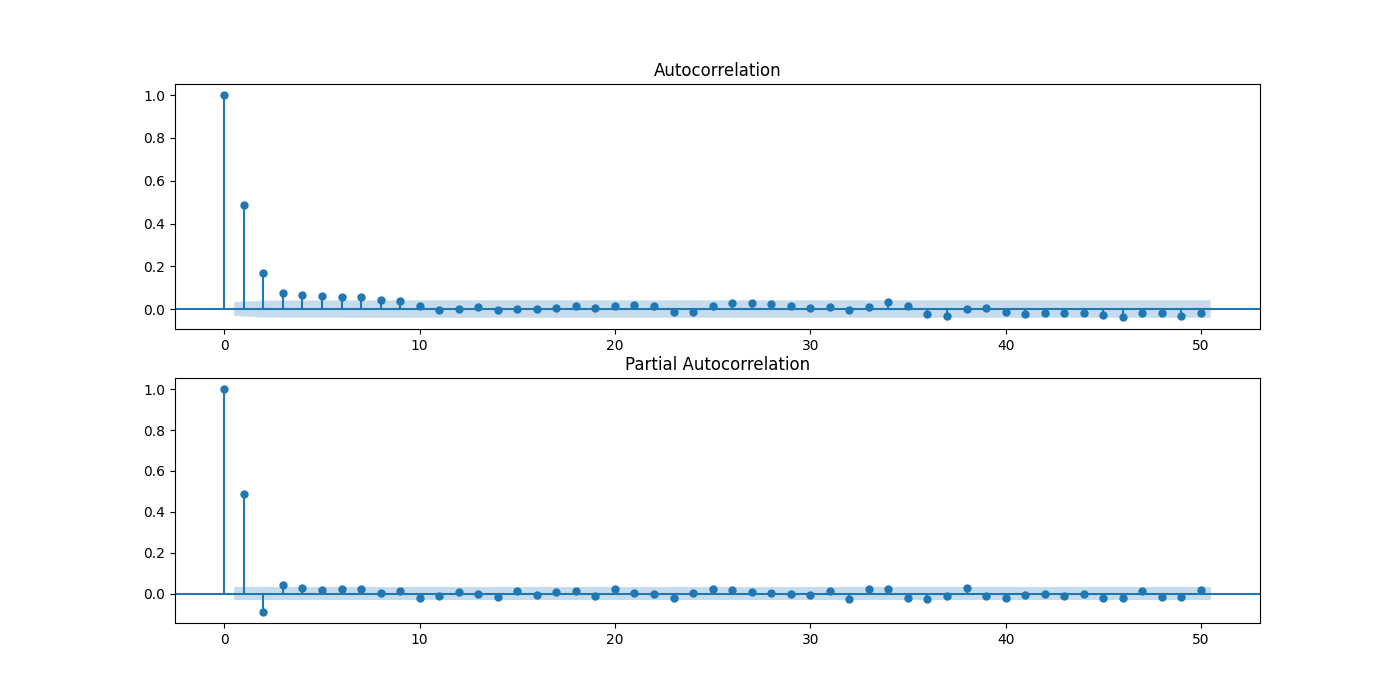
\includegraphics[width=\textwidth]{figures/Ass1/Ass1_D1_PACF_ACF.png}
    \end{minipage}
    \caption{A plot of the \gls{ACF} and \gls{PACF} of the first dataset.}
    \label{fig:Ass1_D1_PACF_ACF}
\end{figure}

\begin{figure}[H]
    \centering
    \begin{minipage}[b]{1\textwidth}
        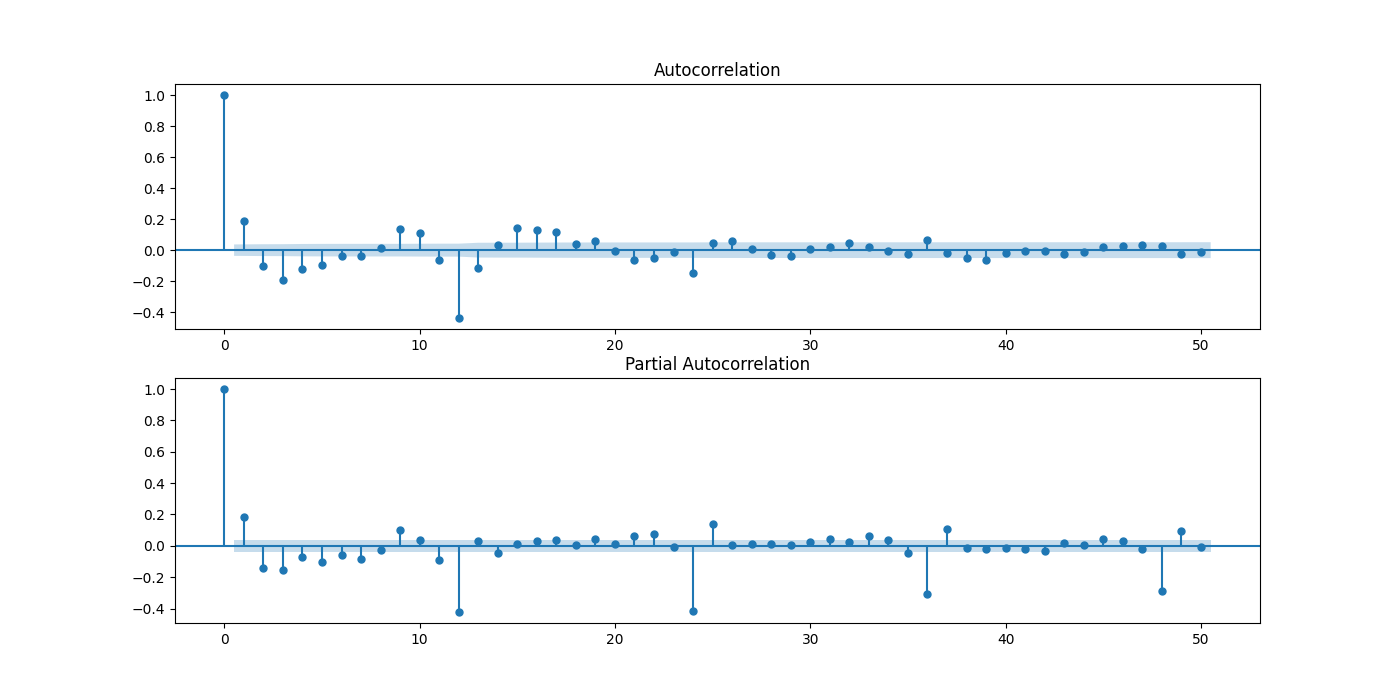
\includegraphics[width=\textwidth]{figures/Ass1/Ass1_D2_PACF_ACF.png}
    \end{minipage}
    \caption{A plot of the \gls{ACF} and \gls{PACF} of the second dataset.}
    \label{fig:Ass1_D2_PACF_ACF}
\end{figure}


\textit{These two plots are used to find the q and p for the ARIMA model. For example, if \gls{ACF} decays towards zero, and \gls{PACF} have only q significant value then our time series is a AR(q) process.}



\textit{The below figures (figures \ref{fig:Ass1_D1_Lag_Plots} and \ref{fig:Ass1_D2_Lag_Plots} ) show the lag plot of the two datasets for different lags. As these plots illustrate, both datasets have diagonal shapes that indicate datasets are not a stationary time series.  }


\begin{figure}[H]
    \centering
    \begin{minipage}[b]{1\textwidth}
        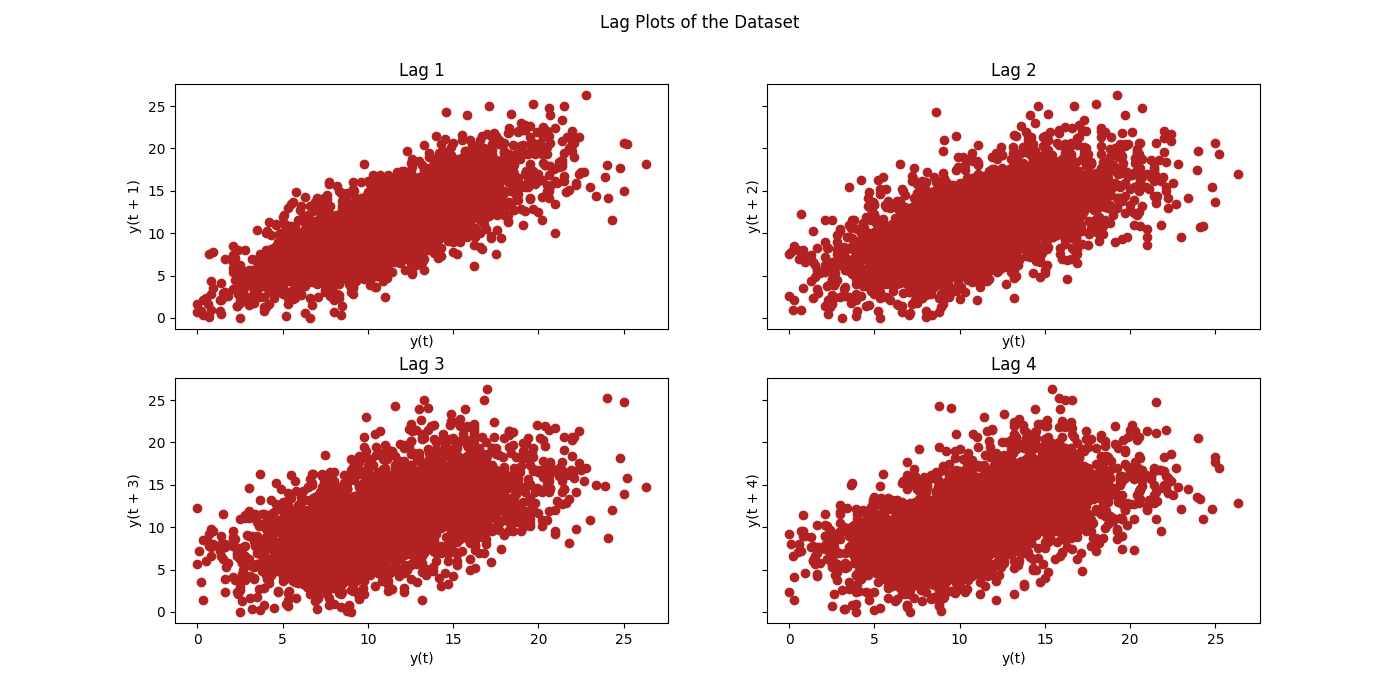
\includegraphics[width=\textwidth]{figures/Ass1/Ass1_D1_Lag_Plots.png}
    \end{minipage}
    \caption{A different lag plot of the first dataset.}
    \label{fig:Ass1_D1_Lag_Plots}
\end{figure}

\begin{figure}[H]
    \centering
    \begin{minipage}[b]{1\textwidth}
        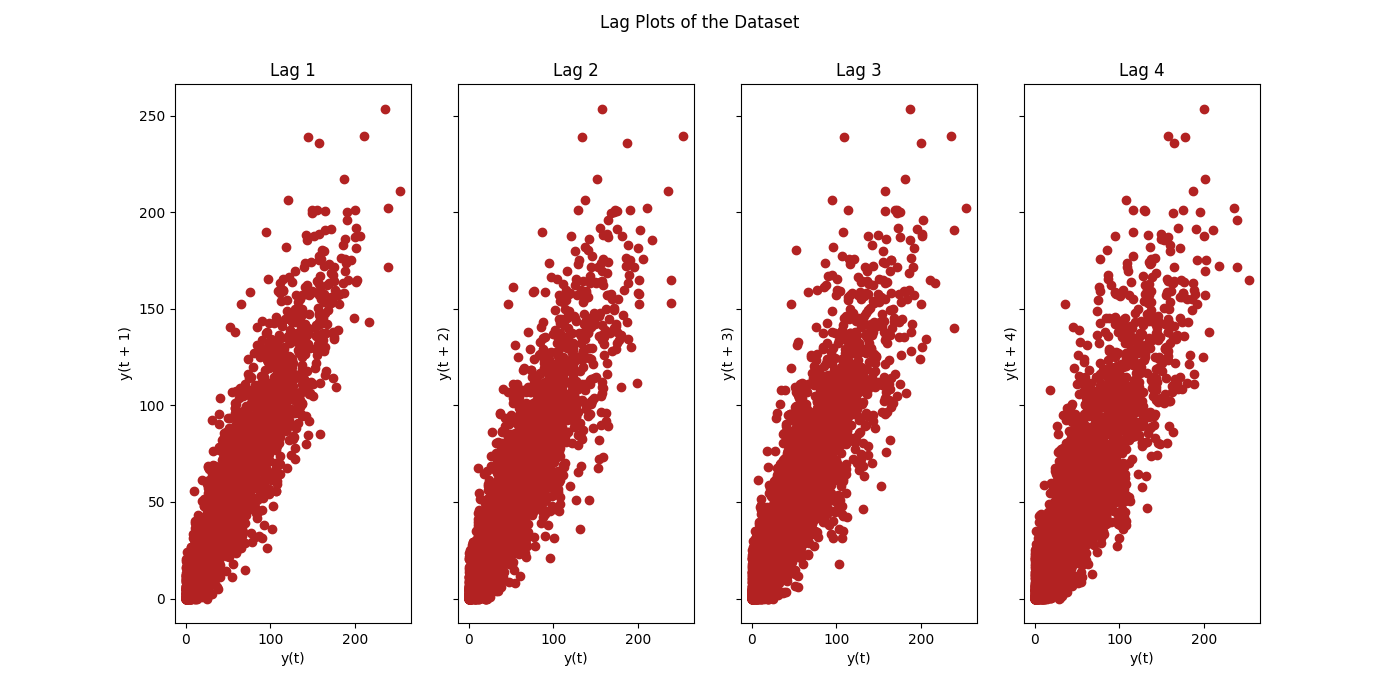
\includegraphics[width=\textwidth]{figures/Ass1/Ass1_D2_Lag_Plots.png}
    \end{minipage}
    \caption{A different lag plot of the second dataset.}
    \label{fig:Ass1_D2_Lag_Plots}
\end{figure}


\textit{Figures \ref{fig:Ass1_D1_Lag_Plots_residual} and \ref{fig:Ass1_D2_Lag_Plots_residual} show the lag plot of the residual component for different lags. As figure \ref{fig:Ass1_D1_Lag_Plots_residual} illustrates, the first dataset has round shapes for lags 2 to 4. Therefore, the time series is stationary for lags 2 to 4 and a weak correlation on lag 1.}

\textit{Figure \ref{fig:Ass1_D2_Lag_Plots_residual} illustrates a clustered around the diagonal that turns to a round shape by increasing the lag. Hence, the dataset has a weak positive autocorrelation. }

\begin{figure}[H]
    \centering
    \begin{minipage}[b]{1\textwidth}
        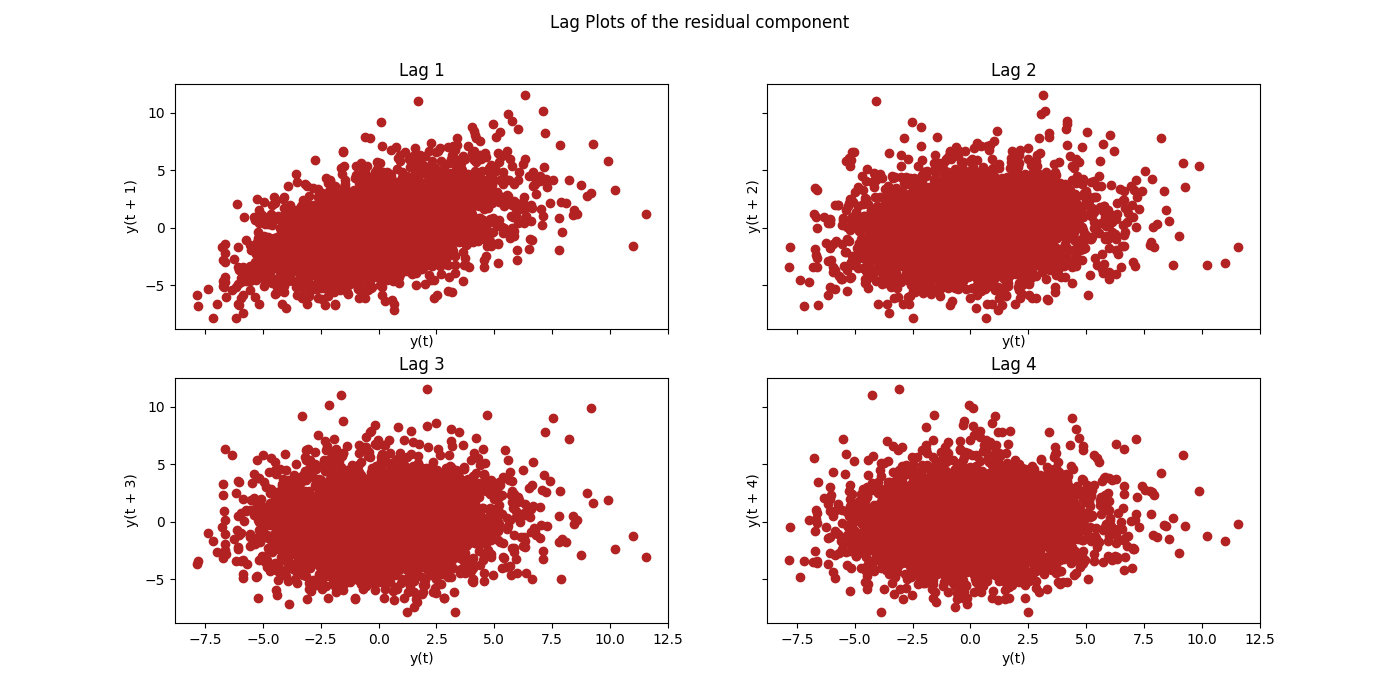
\includegraphics[width=\textwidth]{figures/Ass1/Ass1_D1_Lag_Plots_residual.png}
    \end{minipage}
    \caption{A different lag plot of residual component on the first dataset.}
    \label{fig:Ass1_D1_Lag_Plots_residual}
\end{figure}

\begin{figure}[H]
    \centering
    \begin{minipage}[b]{1\textwidth}
        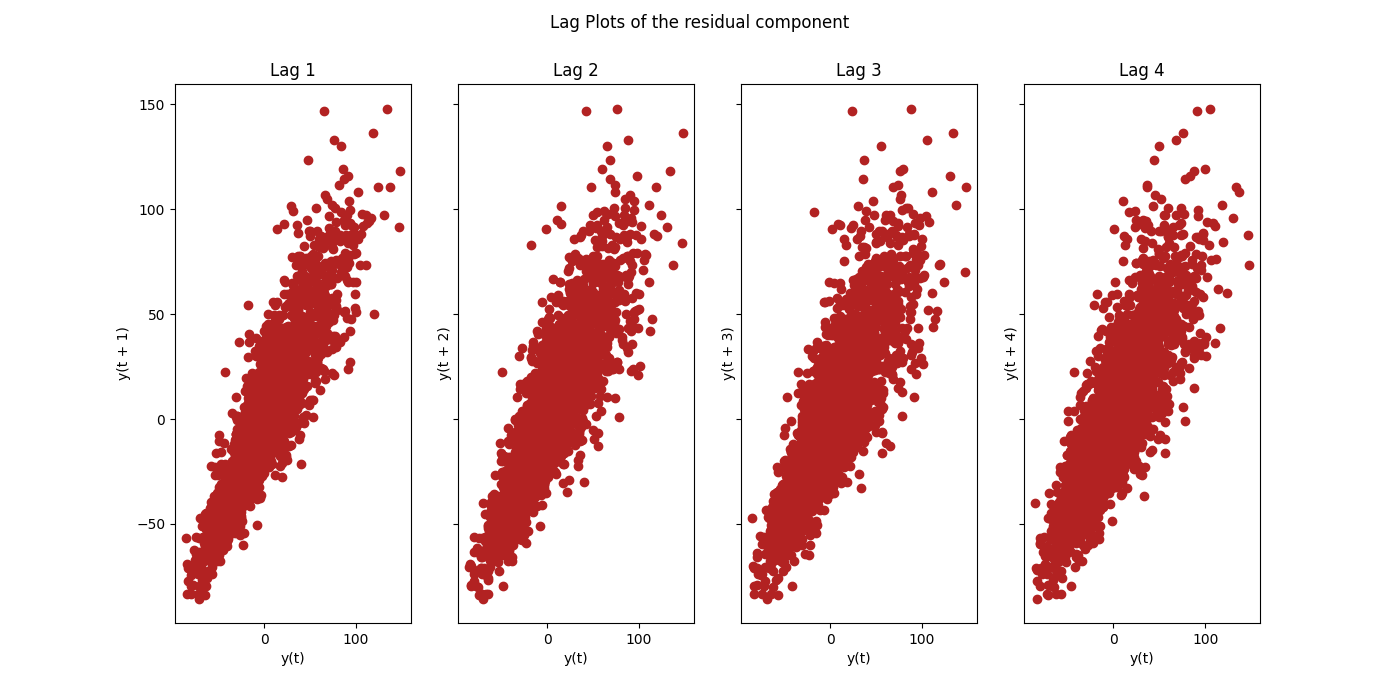
\includegraphics[width=\textwidth]{figures/Ass1/Ass1_D2_Lag_Plots_residual.png}
    \end{minipage}
    \caption{A different lag plot of residual component on the second dataset.}
    \label{fig:Ass1_D2_Lag_Plots_residual}
\end{figure}

\textit{In order to turn the second dataset to a stationary dataset, we can use a first-order differencing. Tables \ref{tab:Ass1_D2_ADF_1_diff} and \ref{tab:Ass1_D2_ADF_1_diff} indicate the result of \gls{ADF} and \gls{KPSS} on the first-order differencing. These two tests show that the data is a stationary dataset.}

\begin{table}[H]
\centering
\caption{The result of the \gls{ADF} test on the $1^{st}$ order differensing in the second dataset.}
\label{tab:Ass1_D2_ADF_1_diff}
\begin{tabular}{lr}
\toprule
{} &             0 \\
\midrule
ADF Statistic               & -8.647591e+00 \\
p-value                     &  5.219691e-14 \\
\#Lags Used                  &  2.300000e+01 \\
Number of Observations Used &  2.795000e+03 \\
Critical Value (1\%)         & -3.432692e+00 \\
Critical Value (5\%)         & -2.862575e+00 \\
Critical Value (10\%)        & -2.567321e+00 \\
\bottomrule
\end{tabular}

\end{table}

\begin{table}[H]
\centering
\caption{The result of the \gls{KPSS} test on the $1^{st}$ order differensing in the second dataset.}
\label{tab:Ass1_D2_KPSS_1_diff}
\begin{tabular}{lr}
\toprule
{} &          0 \\
\midrule
KPSS Statistic        &   0.007892 \\
p-value               &   0.100000 \\
Lags Used             &  54.000000 \\
Critical Value (10\%)  &   0.347000 \\
Critical Value (5\%)   &   0.463000 \\
Critical Value (2.5\%) &   0.574000 \\
Critical Value (1\%)   &   0.739000 \\
\bottomrule
\end{tabular}

\end{table}


\textit{If we look at the \gls{ACF} and \gls{PACF} (figure \ref{fig:Ass1_D2_PACF_ACF_1_diff}),  we can conclude that the data is probably random. Or in other words, there is no autocorrelation between samples. Likewise, figure \ref{fig:Ass1_D2_Lag_Plots_1_diff} confirms this theory.}


\begin{figure}[H]
    \centering
    \begin{minipage}[b]{1\textwidth}
        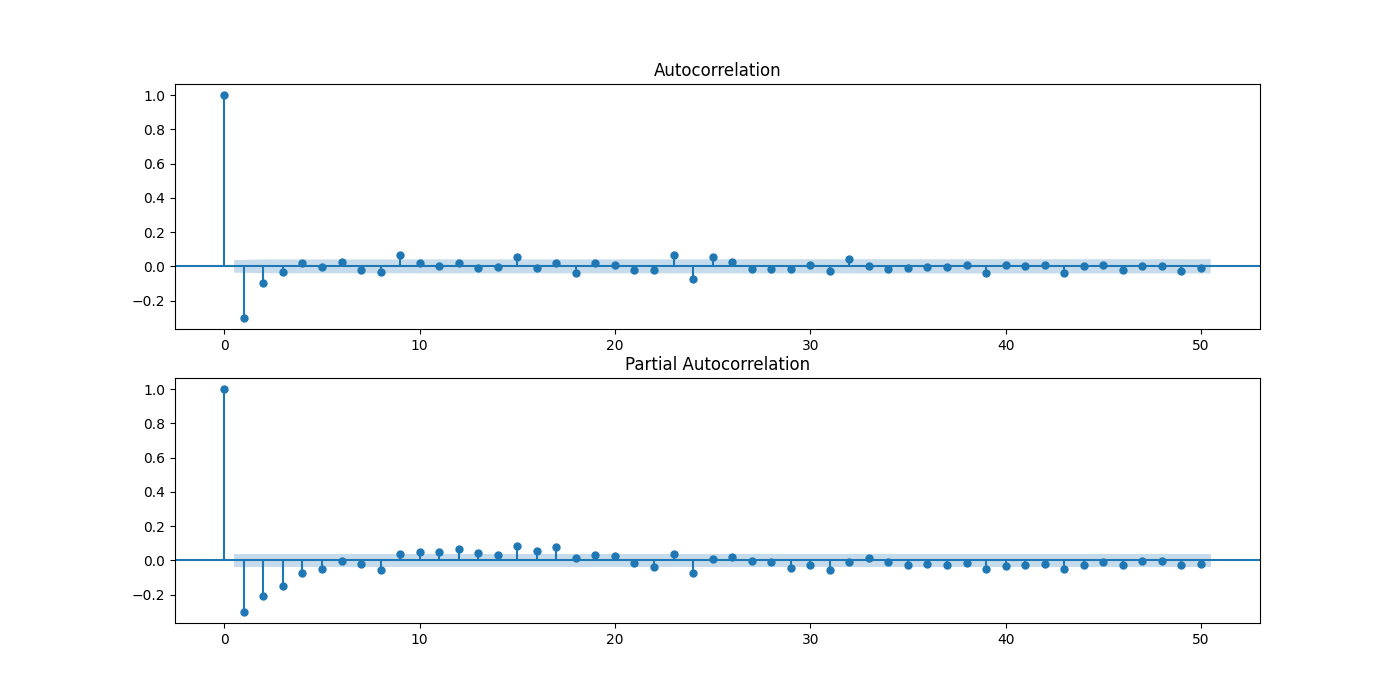
\includegraphics[width=\textwidth]{figures/Ass1/Ass1_D2_PACF_ACF_1_diff.png}
    \end{minipage}
    \caption{A plot of the \gls{ACF} and \gls{PACF} on the $1^{st}$ order differensing.}
    \label{fig:Ass1_D2_PACF_ACF_1_diff}
\end{figure}

\begin{figure}[H]
    \centering
    \begin{minipage}[b]{1\textwidth}
        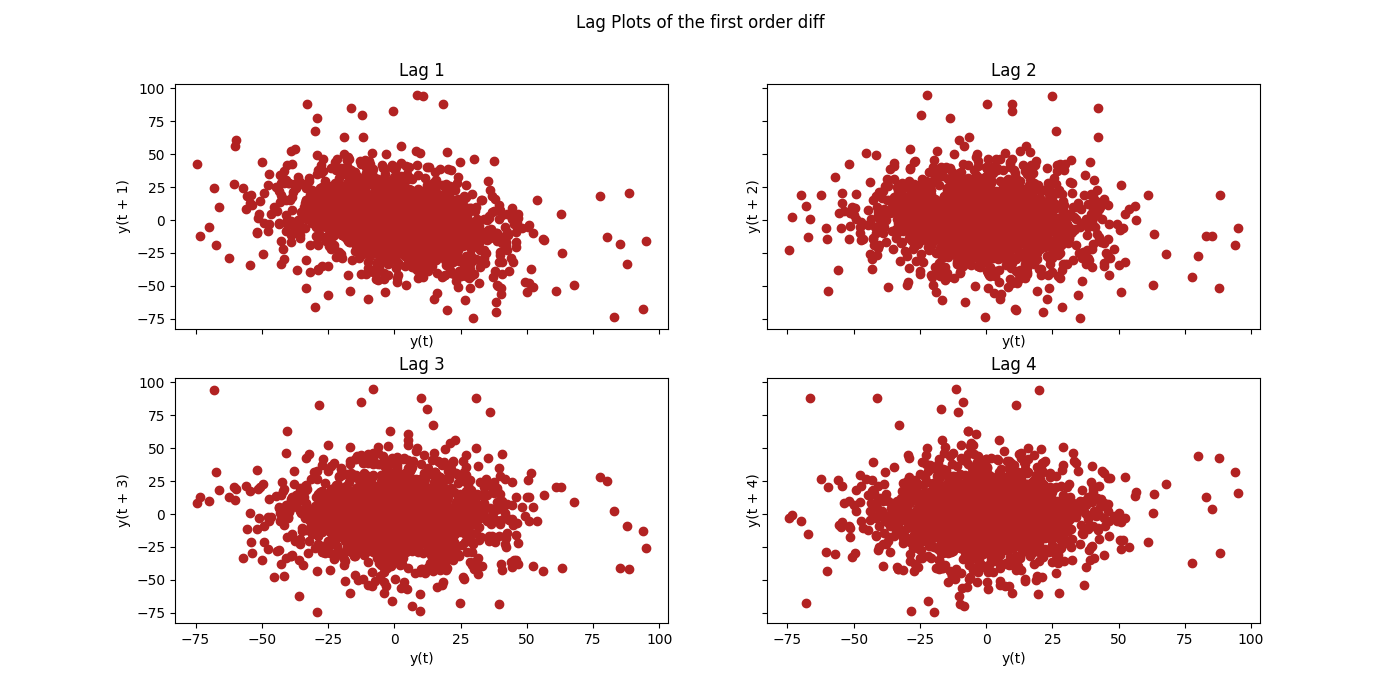
\includegraphics[width=\textwidth]{figures/Ass1/Ass1_D2_Lag_Plots_1_diff.png}
    \end{minipage}
    \caption{A different lag plot on the $1^{st}$ order differensing.}
    \label{fig:Ass1_D2_Lag_Plots_1_diff}
\end{figure}